% !Mode:: "TeX:UTF-8"
%%  本模板推荐以下方式编译:
%%
%%     1. PDFLaTeX[推荐]
%%  注意:
%%   1. 文件默认的编码为 UTF-8 对于windows,请选用支持UTF-8编码的编辑器。
%%   2. 若是模板有什么问题,请及时与我们取得联系,Email:latexstudio@qq.com。
%%   3. 可以到  https://wenda.latexstudio.net 提问
%%   4. 请安装 最新版本的 TeXLive 地址:https://www.latexstudio.net/page/texsoftware/

\documentclass{apmcmthesis}

\usepackage{url}

%%%%%%%%%%%%填写相关信息%%%%%%%%%%%%%%%%%%%%%%%%%%
\tihao{B}                   %选题
\baominghao{90046}           %报名号
\begin{document}
\pagestyle{frontmatterstyle}

\begin{abstract}

\keywords{Keywords1\quad  Keywords2\quad   Keywords3}
\end{abstract}



\newpage
%目录
\tableofcontents


\newpage
\pagestyle{mainmatterstyle}
\setcounter{page}{1}
\section{绪论}

\hspace{2em}Nowadays, leaders and authorities of both countries or regions of a country are seeking ways to improve and boost their regional comprehensive competitiveness. However, the regional comprehensive competitiveness is determined by multiple factors such as economic vitality, living condition and culture depth, which makes it to be a hot topic.

The regional economic vitality is one of the most important part of regional comprehensive competitiveness. Recently, in order to boost the economic vitality, some regions have implemented series of preferential policies to spur the economy vitality. For example, Soochow reduces the investment attraction approval steps and supports the start-ups by providing financial assistance and Wuhan launches policy to lower
the settlement threshold and living cost by up to 20\%  to attract talents. However, due to the existing regional disparity, these policies effect differently. How to seize the key factors and effectively improve the regional economic vitality is really worth studying.

\hspace{2em}In an effort to research the factors influencing economic vitality and how to improve the regional economic vitality, we have acquired some sources along with the given data to build suitable model and solve the problems.
\begin{itemize}
  \item To begin our work, we take Eastern region as an example. We build a relational model involving influencing factors of economic vitality such as the total number of registered enterprises, the amount of residents, regional GDP and so on. Then we study the program of action to improve the regional economic vitality and analyse the effects on the change of regional economic vitality from the perspective of changing trend of population and enterprise vitality.
  \item We continue to use the relational model built in question \textit 1 and the economic vitality measurement index. Then we analyse the short-term and long-term effects on the economic vitality of Eastern region using prediction model when economic policy transformation is implemented. For the population forecast, we adopt the Logistic model. For the quantity of enterprises, we use gray forecast model \textit{GM (1, 1)}. The household consumption, gross domestic production and so on can be classified as economic categories. Therefore, we use time series prediction model based on exponential smoothing to address them.
  \item Evaluating economic vitality is a complicated issue. Therefore, we select a system of 10 indexes that to a large extent can act as measurement of economic vitality and build a measurement model using PCA. Then we rank the economic vitality of cities in \textit{Attachment 3}.
  \item According to the conclusions for Problems \textit{1-3}, we provide an economic development proposal for Eastern region discussed in Problem \textit{2} so that the economic vitality in this region presents the benign sustainable development and its competitiveness is stronger.
\end{itemize}

\section{基本原理}
\subsection{单片机STC89C52}
\begin{itemize}
  \item We assume that the given data and surveyed data are valid and authentic.
  \item We assume that the total number of enterprises in an economic region is the addition of each province in that region.
  \item We assume that the cancellation rate of enterprises in a region is represented by the average rate of each city in that region.
  \item We assume that the selection of factors or indexes that may influence the economic vitality is objective.
  \item We assume that the error or deviation in the data process is within the acceptable range.
\end{itemize}
\subsection{ CC1101模块}
\begin{longtable}{ccp{200pt}}
\toprule
    \textbf{Serial Number} & \textbf{Symbol} & \textbf{Description} \\
\midrule
    \textbf{1}  & \textbf{${A}_{re}$} & The amount of residents in Eastern region within 1 year.\\
    \textbf{2}  & \textbf{${A}_{en}$} & The amount of enterprises in Eastern region within 1 year.\\
    \textbf{3}  & \textbf{${I}_{CPI}$} & The consumer price index in Eastern region within 1 year.\\
    \textbf{4}  & \textbf{${I}_{GDP}$} & The gross domestic product  in Eastern region within 1 year.\\
    \textbf{5}  & \textbf{${I}_{FAI}$} & The fixed-asset investment in Eastern region within 1 year. \\
    \textbf{6}  & \textbf{${I}_{HC}$} & The household consumption in Eastern region within 1 year. \\
    \textbf{7}  & \textbf{${{A}_{10\times 6}}$} & The factor matrix. \\
    \textbf{8}  & \textbf{$R_{6\times6}$} & The correlation coefficient matrix. \\
    \textbf{9}  & \textbf{$Z$} & The comprehensive appraise index. \\
    \textbf{11}  & \textbf{} & 4.88 \\
    \textbf{12} & \textbf{} & 9.71 \\
    \textbf{13} & \textbf{} & 13.97 \\
    \textbf{14} & \textbf{} & 46.68 \\
    \textbf{15} & \textbf{} & 3.03 \\
\bottomrule
\end{longtable}

\section{系统构成与子模块方案选择}
\subsection{单片机 MCU控制模块的最佳方案选择\textit 1}
\hspace{2em}We abstract 6 factors that may affect the economic vitality in Eastern region from the given and surveyed data as follows.
\begin{itemize}
\item The amount of residents in Eastern region from year 2009 to year 2018.
\item The amount of enterprises in Eastern region from year 2009 to year 2018.
\item CPI (consumer price index) in Eastern region from year 2009 to year 2018. 
\item GDP (gross domestic product) in Eastern region from year 2009 to year 2018.
\item FAI (fixed-asset investment) in Eastern region from year 2009 to year 2018.
\item Household consumption in Eastern region from year 2009 to year 2018.
\end{itemize}
\subsubsection{The Amount of Residents}
\hspace{2em}The amount of residents from 2009 to 2018 in each province of Eastern region and the total number are shown in Table \ref{tabel1}. The data is surveyed from \textit{National Bureau of Statistics} (unit: 10000)  
\begin{table}[h]
\scriptsize
\centering
%\captionsetup{font={footnotesize}}
\caption{The amount of residents from 2009 to 2018 in each province of Eastern region and the total number.} 
\begin{tabular}{ccccccccccc}
\toprule
  \textbf{Year} &\textbf{2018} & \textbf{2017} & \textbf{2016} & \textbf{2015} & \textbf{2014} & \textbf{2013} & \textbf{2012} & \textbf{2011} & \textbf{2010} & \textbf{2009}  \\
\midrule
   \textbf{Beijing} & 2154  & 2171  & 2173  & 2171  & 2152  & 2115  & 2069  & 2019  & 1962  & 1860 \\
   \textbf{Tianjin} & 1560  & 1557  & 1562  & 1547  & 1517  & 1472  & 1413  & 1355  & 1299  & 1228  \\
   \textbf{Hebei}   & 7556  & 7520  & 7470  & 7425  & 7384  & 7333  & 7288  & 7241  & 7194  & 7034   \\
   \textbf{Shandong}& 10047 & 10006 & 9947  & 9847  & 9789  & 9733  & 9685  & 9637  & 9588  & 9470\\
   \textbf{Jiangsu} & 8051  & 8029  & 7999  & 7976  & 7960  & 7939  & 7920  & 7899  & 7869  & 7810   \\
   \textbf{Shanghai}& 2424  & 2418  & 2420  & 2415  & 2426  & 2415  & 2380  & 2347  & 2303  & 2210 \\
   \textbf{Zhejiang}& 5737  & 5657  & 5590  & 5539  & 5508  & 5498  & 5477  & 5463  & 5447  & 5276  \\
   \textbf{Fujian}  & 3941  & 3911  & 3874  & 3839  & 3806  & 3774  & 3748  & 3720  & 3693  & 3666    \\
   \textbf{Guangdong}&11346 & 11169 & 10999 & 10849 & 10724 & 10644 & 10594 & 10505 & 10441 & 10130  \\
   \textbf{Hainan}  & 934   & 926   & 917   & 911   & 903   & 895   & 887   & 877   & 869   & 864    \\
   \textbf{Total} & 53750 & 53364 & 52951 & 52519 & 52169 & 51818 & 51461 & 51063 & 50665 & 49548\\
\bottomrule \label{tabel1}
\end{tabular}
\end{table}

We also draw the bar chart of the total number changing from 2009 to 2018 in Figure \ref{residents}.
\begin{figure}[h]
  \centering
  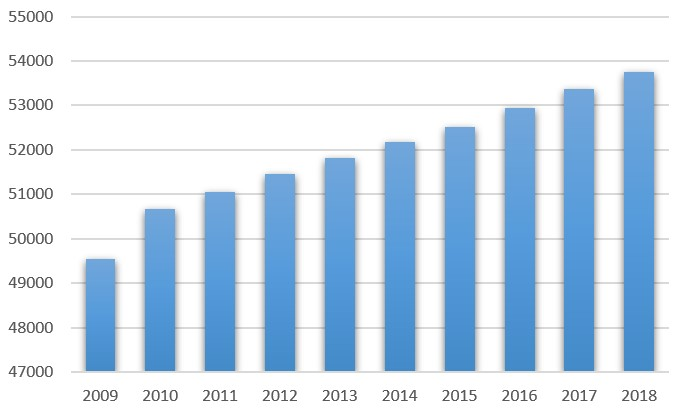
\includegraphics[width=10cm]{residents}
  \caption{The bar chart of the total number changing from 2009 to 2018}\label{residents}
\end{figure}

\subsubsection{The Amount of Enterprises}
\hspace{2em}Cancellation rate can be defined as the ratio of cancelled enterprises to the whole amount of enterprises. Through the cancellation rate we can easily obtain the data of cancelled enterprises. Therefore, based on the amount and increment of enterprises in \textit{Attachments}, the number of surviving enterprises in each year from 2009 to 2018 can be obtained. The amount of surviving enterprises in each year and changing trend from 2009 to 2018 are shown in Figure \ref{enterprises}.
\begin{figure}[h]
  \centering
  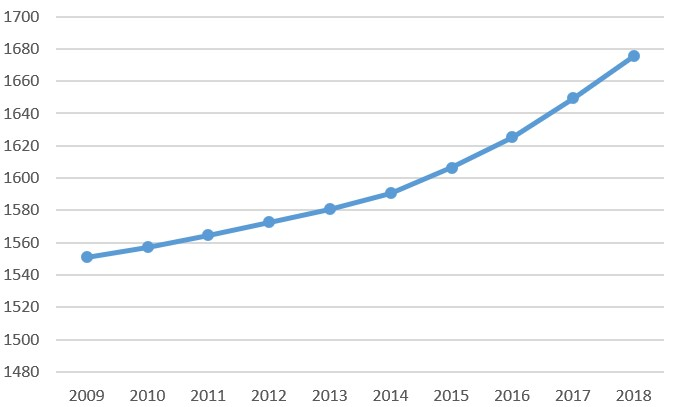
\includegraphics[width=10cm]{enterprises}
  \caption{The line chart of the number of enterprise  changing from 2009 to 2018}\label{enterprises}
\end{figure}
\subsubsection{Consumer Price Index}
\hspace{2em}Consumer price index from 2009 to 2018 in each province of Eastern region and the average number are shown in Table \ref{tabel4}. The data is surveyed from \textit{National Bureau of Statistics} (last year: 100)
\begin{table}[h]
\scriptsize
\centering
%\captionsetup{font={footnotesize}}
\caption{Consumer price index from 2009 to 2018 in each province of Eastern region and the average number.} 
\begin{tabular}{ccccccccccc}
\toprule
  \textbf{Year} &\textbf{2018} & \textbf{2017} & \textbf{2016} & \textbf{2015} & \textbf{2014} & \textbf{2013} & \textbf{2012} & \textbf{2011} & \textbf{2010} & \textbf{2009}  \\
\midrule
   \textbf{Beijing} & 102.50  & 101.90  & 101.40  & 101.80  & 101.60  & 103.30  & 103.30  & 105.60  & 102.40  & 98.50 \\
   \textbf{Tianjin} & 102.00  & 102.10  & 102.10  & 101.70  & 101.90  & 103.10  & 102.70  & 104.90  & 103.50  & 99.00  \\
   \textbf{Hebei}   & 102.40  & 101.70  & 101.50  & 100.90  & 101.70  & 103.00  & 102.60  & 105.70  & 103.10  & 99.30   \\
   \textbf{Shandong}& 102.50  & 101.50  & 102.10  & 101.20  & 101.90  & 102.20  & 102.10  & 105.00  & 102.90  & 100.00 \\
   \textbf{Jiangsu} & 102.30  & 101.70  & 102.30  & 101.70  & 102.20  & 102.30  & 102.60  & 105.30  & 103.80  & 99.60   \\
   \textbf{Shanghai}& 101.60  & 101.70  & 103.20  & 102.40  & 102.70  & 102.30  & 102.80  & 105.20  & 103.10  & 99.60 \\
   \textbf{Zhejiang}& 102.30  & 102.10  & 101.90  & 101.40  & 102.10  & 102.30  & 102.20  & 105.40  & 103.80  & 98.50  \\
   \textbf{Fujian}  & 101.50  & 101.20  & 101.70  & 101.70  & 102.00  & 102.50  & 102.40  & 105.30  & 103.20  & 98.20    \\
   \textbf{Guangdong}&102.20  & 101.50  & 102.30  & 101.50  & 102.30  & 102.50  & 102.80  & 105.30  & 103.10  & 97.70  \\
   \textbf{Hainan}  & 102.50  & 102.80  & 102.80  & 101.00  & 102.40  & 102.80  & 103.20  & 106.10  & 104.80  & 99.30    \\
   \textbf{Average} & 102.18 & 101.82 & 102.13 & 101.53 & 102.08 & 102.63 & 102.67 & 105.38 & 103.37 & 98.97\\
\bottomrule
\end{tabular}\label{tabel4}
\end{table}

We also draw the line chart of the average number changing from 2009 to 2018 in Figure \ref{CPI}.
\begin{figure}[h]
  \centering
  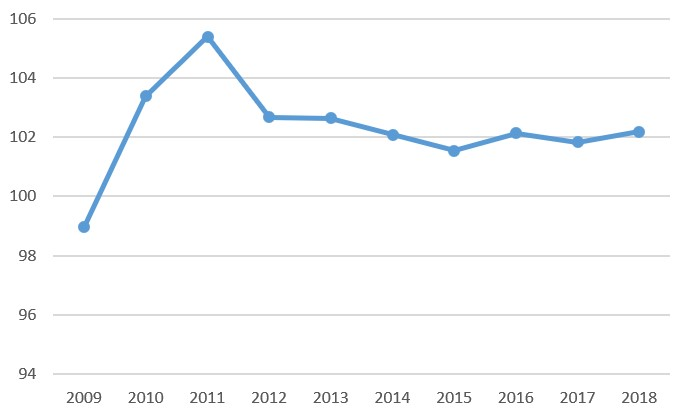
\includegraphics[width=10cm]{CPI}
  \caption{The line chart of the avarage number changing from 2009 to 2018}\label{CPI}
\end{figure}
\subsubsection{Gross Domestic Product}
\hspace{2em}Gross Domestic Product from 2009 to 2018 in each province of Eastern region and the total number are shown in Table \ref{tabel5}. The data is surveyed from \textit{National Bureau of Statistics} (unit: 100 million yuan)
\begin{table}[h]
\scriptsize
\centering
%\captionsetup{font={footnotesize}}
\caption{Gross Domestic Product from 2009 to 2018 in each province of Eastern region and the total number.} 
\begin{tabular}{p{1cm}<{\centering}p{1cm}<{\centering}p{1cm}<{\centering}p{1cm}<{\centering}p{1cm}<{\centering}p{1cm}<{\centering}p{1cm}<{\centering}p{1cm}<{\centering}p{1cm}<{\centering}p{1cm}<{\centering}p{1cm}<{\centering}}
\toprule
  \textbf{Year} &\textbf{2018} & \textbf{2017} & \textbf{2016} & \textbf{2015} & \textbf{2014} & \textbf{2013} & \textbf{2012} & \textbf{2011} & \textbf{2010} & \textbf{2009}  \\
\midrule
   \textbf{Beijing} & 30320 & 28015 & 25669 & 23015 & 21331 & 19801 & 17879 & 16252 & 14114 & 12153 \\
   \textbf{Tianjin} & 18810 & 18550 & 17885 & 16538 & 15727 & 14442 & 12894 & 11307 & 9224 & 7522 \\
   \textbf{Hebei}   & 36010 & 34016 & 32070 & 29806 & 29421 & 28443 & 26575 & 24516 & 20394 & 17235   \\
   \textbf{Shandong}& 76470 & 72634 & 68024 & 63002 & 59427 & 55230 & 50013 & 45362 & 39170 & 33897 \\
   \textbf{Jiangsu} & 92595 & 85870 & 77388 & 70116 & 65088 & 59753 & 54058 & 49110 & 41425 & 34457    \\
   \textbf{Shanghai}& 32680 & 30633 & 28179 & 25123 & 23568 & 21818 & 20182 & 19196 & 17166 & 15046 \\
   \textbf{Zhejiang}& 56197 & 51768 & 47251 & 42886 & 40173 & 37757 & 34665 & 32319 & 27722 & 22990 \\
   \textbf{Fujian}  & 35804 & 32182 & 28811 & 25980 & 24056 & 21868 & 19702 & 17560 & 14737 & 12237   \\
   \textbf{Guangdong}& 97278 & 89705 & 80855 & 72813 & 67810 & 62475 & 57068 & 53210 & 46013 & 39483   \\
   \textbf{Hainan}  & 4832 & 4463 & 4053 & 3703 & 3501 & 3178 & 2856 & 2523 & 2065 & 1654   \\
   \textbf{Total} & 480996  & 447835  & 410186  & 372983 & 350101  & 324765  & 295892  & 271355  & 232031  & 196674\\
\bottomrule
\end{tabular}\label{tabel5}
\end{table}

We also draw the bar chart of the total number changing from 2009 to 2018 in Figure \ref{CPI}.
\begin{figure}[h]
  \centering
  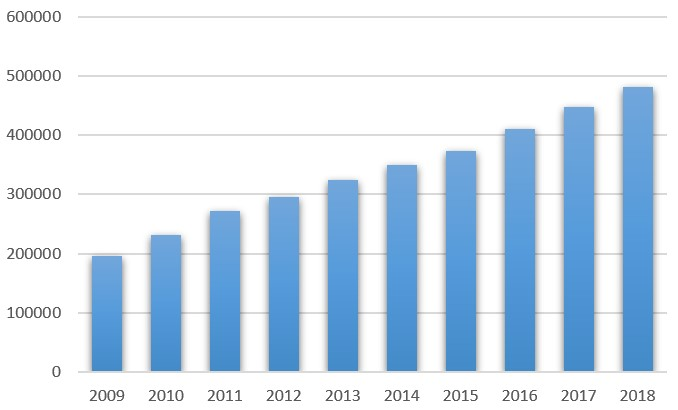
\includegraphics[width=10cm]{GDP}
  \caption{The bar chart of the total number changing from 2009 to 2018}\label{GDP}
\end{figure}


\subsubsection{Fixed-Asset Investment}
\hspace{2em}Fixed-Asset Investment from 2009 to 2018 in each province of Eastern region and the total number are shown in Table \ref{tabel6}. The data of 2018 is predicted with data of previous years with an error within 5\%. The data is surveyed from \textit{National Bureau of Statistics} (unit: 100 million yuan)
\begin{table}[h]
\scriptsize
\centering
%\captionsetup{font={footnotesize}}
\caption{Fixed-Asset Investment from 2009 to 2018 in each province of Eastern region and the total number.} 
\begin{tabular}{p{1cm}<{\centering}p{1cm}<{\centering}p{1cm}<{\centering}p{1cm}<{\centering}p{1cm}<{\centering}p{1cm}<{\centering}p{1cm}<{\centering}p{1cm}<{\centering}p{1cm}<{\centering}p{1cm}<{\centering}p{1cm}<{\centering}}
\toprule
  \textbf{Year} &\textbf{2018} & \textbf{2017} & \textbf{2016} & \textbf{2015} & \textbf{2014} & \textbf{2013} & \textbf{2012} & \textbf{2011} & \textbf{2010} & \textbf{2009}  \\
\midrule
   \textbf{Beijing} & 8862  & 8370  & 7944  & 7496  & 6924  & 6847  & 6112  & 5579  & 5403  & 4617 \\
   \textbf{Tianjin} & 13881  & 11289  & 12779  & 11832  & 10518  & 9130  & 7935  & 7068  & 6278  & 4738 \\
   \textbf{Hebei}   & 37070  & 33407  & 31750  & 29448  & 26672  & 23194  & 19661  & 16389  & 15083  & 12270   \\
   \textbf{Shandong}& 61480  & 55203  & 53323  & 48312  & 42496  & 36789  & 31256  & 26750  & 23281  & 19035 \\
   \textbf{Jiangsu} & 58598  & 53277  & 49663  & 46247  & 41939  & 36373  & 30854  & 26693  & 23184  & 18950    \\
   \textbf{Shanghai}& 7258  & 7247  & 6756  & 6353  & 6016  & 5648  & 5118  & 4962  & 5109  & 5044 \\
   \textbf{Zhejiang}& 35233  & 31696  & 30276  & 27323  & 24263  & 20782  & 17649  & 14185  & 12376  & 10742 \\
   \textbf{Fujian}  & 35233  & 26416  & 23237  & 21301  & 18178  & 15327  & 12440  & 9911  & 8199  & 6231   \\
   \textbf{Guangdong}& 39358  & 37762  & 33304  & 30343  & 26294  & 22308  & 18752  & 17069  & 15624  & 12933   \\
   \textbf{Hainan}  & 4720  & 4244  & 3890  & 3451  & 3112  & 2698  & 2145  & 1657  & 1317  & 988   \\
   \textbf{Total} & 301693  & 268911  & 252923  & 232107  & 206412  & 179098  & 151923  & 130263  & 115854  & 95548\\
\bottomrule
\end{tabular}\label{tabel6}
\end{table}

We also draw the line chart of the total number changing from 2009 to 2018 in Figure \ref{FAI}.
\begin{figure}[h]
  \centering
  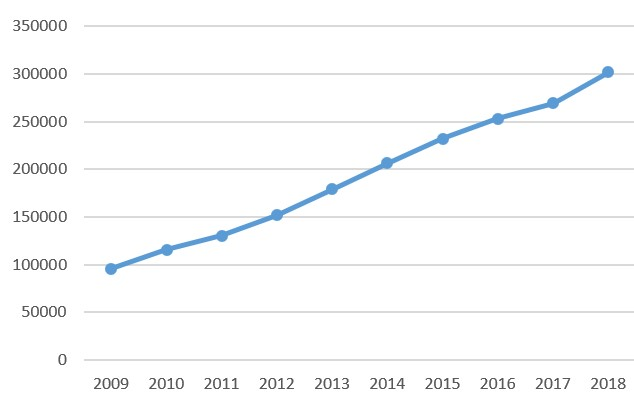
\includegraphics[width=10cm]{FAI}
  \caption{The line chart of the total number changing from 2009 to 2018}\label{FAI}
\end{figure}

\subsubsection{Household Consumption}
\hspace{2em}Household Consumption from 2009 to 2018 in each province of Eastern region and the total number are shown in Table \ref{tabel7}. The data of 2018 is predicted with data of previous years with an error within 5\%. The data is surveyed from \textit{National Bureau of Statistics} (unit: yuan)
\begin{table}[h]
\scriptsize
\centering
%\captionsetup{font={footnotesize}}
\caption{Fixed-Asset Investment from 2009 to 2018 in each province of Eastern region and the total number.} 
\begin{tabular}{p{1cm}<{\centering}p{1cm}<{\centering}p{1cm}<{\centering}p{1cm}<{\centering}p{1cm}<{\centering}p{1cm}<{\centering}p{1cm}<{\centering}p{1cm}<{\centering}p{1cm}<{\centering}p{1cm}<{\centering}p{1cm}<{\centering}}
\toprule
  \textbf{Year} &\textbf{2018} & \textbf{2017} & \textbf{2016} & \textbf{2015} & \textbf{2014} & \textbf{2013} & \textbf{2012} & \textbf{2011} & \textbf{2010} & \textbf{2009}  \\
\midrule
   \textbf{Beijing} & 53710  & 52912  & 48883  & 39200  & 36057  & 33337  & 30350  & 27760  & 24982  & 22023 \\
   \textbf{Tianjin} & 41563  & 38975  & 36257  & 32595  & 28492  & 26261  & 22984  & 20624  & 17852  & 15200 \\
   \textbf{Hebei}   & 16502  & 15893  & 14328  & 12829  & 12171  & 11557  & 10749  & 9551  & 8057  & 7193   \\
   \textbf{Shandong}& 28998  & 28353  & 25860  & 20684  & 19184  & 16728  & 15095  & 13524  & 11606  & 10494 \\
   \textbf{Jiangsu} & 42541  & 39796  & 35875  & 31682  & 28316  & 23585  & 19452  & 17167  & 14035  & 11993    \\
   \textbf{Shanghai}& 55861  & 53617  & 49617  & 45816  & 43007  & 39223  & 36893  & 35439  & 32271  & 26582 \\
   \textbf{Zhejiang}& 35487  & 33851  & 30743  & 28712  & 26885  & 24771  & 22845  & 21346  & 18274  & 15867  \\
   \textbf{Fujian}  & 26643  & 25969  & 23355  & 20828  & 19099  & 17115  & 16144  & 14958  & 13187  & 11336   \\
   \textbf{Guangdong}& 32444  & 30762  & 28495  & 26365  & 24582  & 23739  & 21823  & 19578  & 17211  & 15243   \\
   \textbf{Hainan}  & 21747  & 20939  & 18431  & 17019  & 12915  & 11712  & 10634  & 9238  & 7553  & 6695  \\
   \textbf{Total} & 355496  & 341067  & 311844  & 275730  & 250708  & 228028  & 206969  & 189185  & 165028  & 142626\\
\bottomrule
\end{tabular}\label{tabel7}
\end{table}

We also draw the bar chart of the total number changing from 2009 to 2018 in Figure \ref{HC}.
\begin{figure}[h]
  \centering
  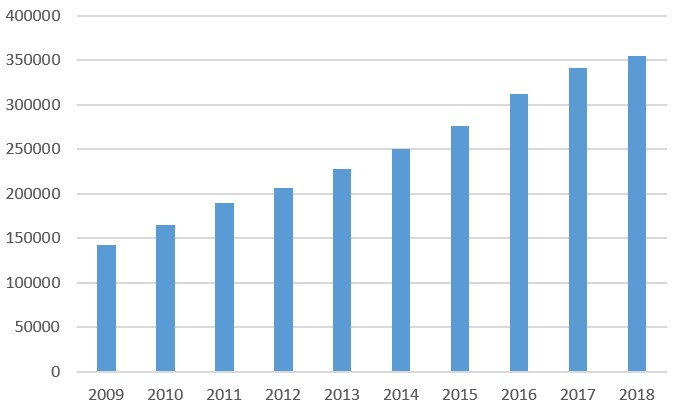
\includegraphics[width=10cm]{HC}
  \caption{The bar chart of the total number changing from 2009 to 2018}\label{HC}
\end{figure}



\subsection{无线通信模块的方案选择 \textit 1}
\subsubsection{ 无线通信模块可选择的方案}
\hspace{2em}According to question \textit 1 and the results of data process, we adopt the method PCA to build the relational model to measure the economic vitality and influencing factors in Eastern region. We give the details of model construction by steps using PCA as follows.

1) Firstly, we use the results of 6 factor variables from data process to create the factor matrix ${{A}_{10\times 6}}$ which is defined in the following equation.
\begin{equation}
A=(a_{ij})_{10\times 6}
\end{equation}
where the integer $i$ ranges from 1 to 10 representing year from 2009 to 2018 and the integer $j$ ranges from 1 to 6 representing factors \textit{household consumption, FAI, GDP, CPI, the amount of residents and the amount of enterprises} respectively. Therefore, the factor variables can be symbolized as $x_j$.

2) Secondly, we normalize each element value in the factor matrix using the following equation.
\begin{equation}
{{\tilde{a}}_{ij}}=\frac{{{a}_{ij}}-{{\mu }_{j}}}{{{s}_{j}}}
\end{equation}
\begin{equation}
{{\mu }_{j}}=\frac{1}{10}\sum\limits_{i=1}^{10}{{{a}_{ij}}}
\end{equation}
\begin{equation}
{{s}_{j}}=\sqrt{\frac{1}{9}\sum\limits_{i=1}^{10}{{{({{a}_{ij}}-{{\mu }_{j}})}^{2}}}}
\end{equation}
(3) and (4) are the sample mean value and the sample standard deviation of $j$th factor respectively. Accordingly, the factor variables $x_j$ can be normalized as ${{\tilde{x_j}}}$ with the following equation.
\begin{equation}
{{\tilde{x}}_{j}}=\frac{{{x}_{j}}-{{\mu }_{j}}}{{{s}_{j}}}
\end{equation}

3) Thirdly, we formulate the correlation coefficient matrix $R$ with the following equation.
\begin{equation}
R=({{r}_{{{j}_{1}}{{j}_{2}}}})_{6\times 6}
\end{equation}
\begin{equation}
{{r}_{{{j}_{1}}{{j}_{2}}}}=\frac{\sum\limits_{i=1}^{10}{{{{\tilde{a}}}_{i{{j}_{1}}}}}\centerdot {{{\tilde{a}}}_{i{{j}_{2}}}}}{9}
\end{equation}
where $j_1$ and $j_2$, with different value from 1 to 6, are the same as $j$. ${{r}_{{{j}_{1}}{{j}_{2}}}}$ is the correlation coefficient of $j_1$th factor and $j_2$th factor and also the element of correlation coefficient matrix.

4) Fourthly, we calculate the feature values $\lambda_j$ (${\lambda_j}\ge0$) and corresponding normalized feature vectors ${{[{{u}_{1j}},{{u}_{2j}},\ldots ,{{u}_{6j}}]}^{T}}$ of correlation coefficient matrix $R$. Then the principal components formed by 6 normalized feature vectors are formulated as follows.
\begin{equation}
\left\{ \begin{array}{*{35}{l}}
   {{y}_{1}}={{u}_{11}}{{{\tilde{x}}}_{1}}+{{u}_{21}}{{{\tilde{x}}}_{2}}+\ldots +{{u}_{61}}{{{\tilde{x}}}_{6}}  \\
   {{y}_{2}}={{u}_{12}}{{{\tilde{x}}}_{1}}+{{u}_{22}}{{{\tilde{x}}}_{2}}+\ldots +{{u}_{62}}{{{\tilde{x}}}_{6}}  \\
   {{y}_{3}}={{u}_{13}}{{{\tilde{x}}}_{1}}+{{u}_{23}}{{{\tilde{x}}}_{2}}+\ldots +{{u}_{63}}{{{\tilde{x}}}_{6}}  \\
   {{y}_{4}}={{u}_{14}}{{{\tilde{x}}}_{1}}+{{u}_{24}}{{{\tilde{x}}}_{2}}+\ldots +{{u}_{64}}{{{\tilde{x}}}_{6}}  \\
   {{y}_{5}}={{u}_{15}}{{{\tilde{x}}}_{1}}+{{u}_{25}}{{{\tilde{x}}}_{2}}+\ldots +{{u}_{65}}{{{\tilde{x}}}_{6}}  \\
   {{y}_{6}}={{u}_{16}}{{{\tilde{x}}}_{1}}+{{u}_{26}}{{{\tilde{x}}}_{2}}+\ldots +{{u}_{66}}{{{\tilde{x}}}_{6}}  \\
\end{array} \right.
\end{equation}
where $y_j$ denotes the $j$th principal component.

5) Fifthly, we select $p$ out of 6 principal components to measure their comprehensive appraisal value. Contribution rate $b_j$ of each feature value $\lambda_j$ is also the contribution rate of corresponding principal component $y_j$, which is formulated as follows.
\begin{equation}
{{b}_{j}}=\frac{{{\lambda }_{j}}}{\sum\limits_{j=1}^{6}{{{\lambda }_{j}}}}
\end{equation}
Then the accumulation contribution rate of $p$ principal components can be formulated as follows.
\begin{equation}
{{\partial }_{p}}=\frac{\sum\limits_{j=1}^{p}{{{\lambda }_{j}}}}{\sum\limits_{j=1}^{6}{{{\lambda }_{j}}}}
\end{equation}
If $\partial_p$ approximates 1, it means that we can choose these $p$ principal components to substitute for the original 6 principal components. The comprehensive appraise of principal components is then simplified.

6) Lastly, the result of comprehensive appraise $Z$ can be acquired through computation. The following equation gives the formulation of $z$.
\begin{equation}
Z=\sum\limits_{j=1}^{p}{{{b}_{j}}{{y}_{j}}}
\end{equation}
\subsubsection{无线通信模块的最佳方案分析}
\hspace{2em}Based on the model constructed using PCA, we apply Matlab to produce the model results. Primarily we select all of the 6 normalized factor variables deviated from the original factor variables and obtain the 6 principal components. Then we figure out the weight of each normalized factor variable to the 6 principal components through computation and the numbers in Table \ref{table2} show them clearly.
\begin{table}[h]
\centering
\footnotesize
%\captionsetup{font={footnotesize}}
\caption{Weight of each normalized factor variable to the principal components.}
\begin{tabular}{ccccccc}
\toprule
\textbf{Principal Component}& \textbf{${\tilde{x}}_{1}$}&\textbf{${\tilde{x}}_{2}$}&\textbf{${\tilde{x}}_{3}$}&\textbf{${\tilde{x}}_{4}$}&\textbf{${\tilde{x}}_{5}$}&\textbf{${\tilde{x}}_{6}$}\\
\midrule
\textbf{$y_1$} & 0.4502 & -0.0182 &-0.0287 &-0.7079 &0.4598 &-0.2893\\
\textbf{$y_2$} & 0.4491 & -0.0504 &-0.2367 &0.6360  &0.5734 &0.0806\\
\textbf{$y_3$} & 0.4503 & 0.0272  &-0.1160 &-0.2181 &-0.2708&0.8137\\
\textbf{$y_4$} & -0.0052 & 0.9875 &0.1112  &0.0244  &0.1058 &0.0275\\
\textbf{$y_5$} & 0.4447 & 0.1262  &-0.4518 &0.1144  &-0.5834&-0.4782\\
\textbf{$y_6$} & 0.4417 & -0.0735 &0.8445  &0.1823  &-0.1869&-0.1349\\
\bottomrule\label{table2}
\end{tabular}
\end{table}

Afterwards, the contribution rates and the accumulation contribution rates of each principal component to the comprehensive appraise index $Z$ are shown in Table \ref{table3} 
\begin{table}[h]
\centering
\footnotesize
%\captionsetup{font={footnotesize}}
\caption{Contribution rates and accumulation contribution rates of each principal component to the comprehensive appraise index.}
\begin{tabular}{|c|c|c|}
\hline
\textbf{Principal Component}&\textbf{Contribution Rate (\%)}& \textbf{Accumulation Contribution Rate (\%)}\\
\hline
\textbf{$y_1$} & 81.9304 & 81.9304 \\
\hline
\textbf{$y_2$} & 17.0794 & 99.0098 \\
\hline
\textbf{$y_3$} & 0.8233  & 99.8331 \\
\hline
\textbf{$y_4$} & 0.0805   & 99.9136 \\
\hline
\textbf{$y_5$} & 0.0581  & 99.9717 \\
\hline
\textbf{$y_6$} & 0.0283  & 100.0000 \\
\hline
\end{tabular}\label{table3}
\end{table}

Based on the results shown in Table \ref{table2} and Table \ref{table3}, we finally select the first 3 principal components instead of the original 6 principal components according to their contribution rates and accumulation contribution rates and also we add up the weights of the 6 normalized factor variables to the first 3 principal components. The final result, also the relational model of influencing factors, is formulated as follows.
\begin{equation}
Z=0.4824{\tilde{x}}_{1}-0.0213{\tilde{x}}_{2}-0.0735{\tilde{x}}_{3}-0.4889{\tilde{x}}_{4}+0.4524{\tilde{x}}_{5}-0.0497{\tilde{x}}_{6}
\end{equation}
where ${\tilde{x}}_{1}$, ${\tilde{x}}_{2}$, ${\tilde{x}}_{3}$, ${\tilde{x}}_{4}$, ${\tilde{x}}_{5}$ and ${\tilde{x}}_{6}$ denote to household consumption, FAI, GDP, CPI, the amount of residents and the amount of enterprises respectively.


\subsection{总体方案设计}
\subsubsection{设计1}
\hspace{2em}In a short term, the growth of residents will benefit the economy in terms of labour resource and skilled talents. However, the restriction from limited living room and finite natural resources will constrain the resident growth. Therefore, we propose to use Logistic Model to predict the population growth of residents and give the detailed steps.

1) The population is a function of year $i$ and can be formed as $n(i)$. The growth rate $r$ is a function of population and can then be described as a decrement function $r(n)$. We suppose $r(n)$ is a linear function and is formulated as follows.
\begin{equation}
r(n)=r-sn
\end{equation}
where $s$ is a coefficient. Assumption is made that the maximum population which Eastern region can hold is $n_{max}$. That means when the population reaches the maximum the growth rate reduces to nearly 0.

2) Based on the above model assumption, we further formulate the growth rate as follows.
\begin{equation}
r(n)=r(1-{\frac{n}{n_{max}}})
\end{equation}
Logistic model is built and shown as follows.
\begin{equation}
\left\{ \begin{array}{*{35}{l}}
   \frac{dn}{di}=n\centerdot r(1-\frac{n}{{{n}_{\max }}})  \\
   n({{i}_{0}})={{n}_{0}}  \\
\end{array} \right. 
\end{equation}
where $i_0$ and $n_0$ are the initial value of year and population respectively. The solution to Equations (15) is as follows.
\begin{equation}
n(i)=\frac{{{n}_{\max }}}{1+(\frac{{{n}_{\max }}}{{{n}_{0}}}-1){{e}^{-r(i-{{i}_{0}})}}}
\end{equation}

3) Based on the solution given above, we import data in \textit{Excel} to \textit{Matlab} and get the prediction results of resident population in next years.
\subsubsection{设计2}
\hspace{2em}Based on the background, we plan to apply commonly used \textit{GM(1,1)} to predict the quantity of enterprises in next years. We give the steps of model construction.

1) Firstly, we test the data of enterprise quantity. The primary data sequence is $m^{(0)}$ and
\begin{equation}
m^{(0)}=[m^{(0)}(1), m^{(0)}(2), m^{(0)}(3),......, m^{(0)}(i)]
\end{equation}
where $i$ is year. The sequence ratio $\lambda(k)$ is define as follows.
\begin{equation}
\lambda (k)=\frac{{{m}^{(0)}}(k-1)}{{{m}^{(0)}}(k)}
\end{equation}
where $k$ equals $i$ and starts from 2. The range of sequence ratio $(1.0040, 1.0158)$ is obtained through \textit{Matlab} and justifies the use of \textit{GM(1,1)} by covering the following range.
\begin{equation}
\Theta=(e^{-\frac{2}{\pi}}, e^{\frac{1}{6}})=(0.834, 1.181)
\end{equation} 

2) Secondly, we obtain $m^{(1)}$ through the following equation.
\begin{equation}
{{m}^{(1)}}=[{{m}^{(0)}}(1),\sum\limits_{k=1}^{2}{{{m}^{(0)}}(k)},\sum\limits_{k=1}^{3}{{{m}^{(0)}}(k)},......,\sum\limits_{k=1}^{10}{{{m}^{(0)}}(k)}]
\end{equation}
Then the data matrix $B$ and the data column vector $Y$ are formulated as
\begin{equation}
B=\left[ \begin{matrix}
   -\frac{1}{2}[{{m}^{(1)}}(1)+{{m}^{(1)}}(2)] & 1  \\
   -\frac{1}{2}[{{m}^{(1)}}(2)+{{m}^{(1)}}(3)] & 1  \\
   \vdots  & \vdots   \\
   -\frac{1}{2}[{{m}^{(1)}}(9)+{{m}^{(1)}}(10)] & 1  \\
\end{matrix} \right]
, 
Y=\left[ \begin{matrix}
   {{m}^{(0)}}(2)  \\
   {{m}^{(0)}}(3)  \\
   \vdots   \\
   {{m}^{(0)}}(10)  \\
\end{matrix} \right]
\end{equation}

3) Thirdly, \textit{GM(1,1)} is built and shown as follows.
\begin{equation}
\left\{ \begin{array}{*{35}{l}}
   \frac{d{{m}^{(1)}}}{di}+\hat{a}{{m}^{(1)}}=\hat{b}  \\
   \hat{u}=\left[ \begin{array}{*{35}{l}}
   {\hat{a}}  \\
   {\hat{b}}  \\
\end{array} \right]={{({{B}^{T}}B)}^{-1}}{{B}^{T}}Y  \\
\end{array} \right.
\end{equation}
The solution is
\begin{equation}
{{\hat{m}}^{(1)}}(k+1)=[{{m}^{(0)}}(1)-\frac{{\hat{b}}}{{\hat{a}}}]{{e}^{-\hat{a}k}}+\frac{{\hat{b}}}{{\hat{a}}}
\end{equation}

4) Fourthly, We import the data of enterprises to \textit{Matlab} and get the fitting results shown in Figure \ref{}.

5) Finally, we test our model using sequence ratio deviation         $p(k)$. We calculate the sequence ratio $\lambda(k)$ with reference data $m^{(0)}(k-1)$ and $m^{(0)}(k)$. Therefore, the sequence ratio deviation is formulated as follows.
\begin{equation}
p(k)=1-(\frac{1-0.5a}{1+0.5a})\centerdot \lambda (k)
\end{equation}
The final sequence ratio deviation is $0.18261$ and less than $0.2$. The prediction results meet the requirement.
\subsubsection{she'ji}
\hspace{2em}Based on previous analysis, we classify CPI, GDP, FAI and household consumption as economic category , compared with the other two factors. Commonly, the effect of history data on prediction usually fades away as time proceeds. Therefore, a better and more practical way to predict the value of these factors is applying weight which decreases with time to history data in the prediction work. We then choose to apply second-exponential smoothing model and discuss the details in model construction by steps.

1) Firstly, the exponential smoothing model is formulated as 
\begin{equation}
S_{i}^{(1)}=\alpha {{e}_{i}}+(1-\alpha )e_{i-1}^{(1)}=e_{i-1}^{(1)}+\alpha ({{e}_{i}}-S_{i-1}^{(1)})
\end{equation}
where $e_i$ and $\alpha$ are time sequence of factors and weighted coefficient respectively. The integer $i$ ranges from 1 to 10 representing year from 2009 to 2018 and $\alpha$ is from 0 to 1. The iteration of moving average is 
\begin{equation}
\mu _{i}^{(1)}=\mu _{i-1}^{(1)}+\frac{{{e}_{i}}-{{e}_{i-N}}}{N}
\end{equation}
where $\alpha$ equals $\frac{1}{N}$. We then choose $\mu _{i-1}^{(1)}$ to be the best estimation of $e_{i-N}$ and get the following equation.
\begin{equation}
\mu _{i}^{(1)}=\mu _{i-1}^{(1)}+\frac{{{e}_{i}}-\mu _{i-1}^{(1)}}{N}=\frac{{{e}_{i}}}{N}+(1-\frac{1}{N})\mu _{i-1}^{(1)}
\end{equation}
We replace $\mu _{i}^{(1)}$ with $S_i$ and get the following equation.
\begin{equation}
S_{i}^{(1)}=\alpha {{e}_{i}}+(1-\alpha )S_{i-1}^{(1)}
\end{equation}
That means $S_i^{(1)}$ is the weighted average of all history data with the weighted coefficient to be $\alpha$, $\alpha(1-\alpha)$, $\alpha(1-\alpha)^2$ and so on. Obviously, the following equation is established.
\begin{equation}
{{\sum\limits_{k=0}^{\infty }{\alpha (1-\alpha )^{k}}}}=\frac{\alpha }{1-(1-\alpha )}=1
\end{equation}
Then the prediction model can be further formulated as
\begin{equation}
{{\hat{e}}_{i+1}}=S_{i}^{(1)}=\alpha {{e}_{i}}+(1-\alpha ){{\hat{e}}_{i}}
\end{equation}

2) Secondly, we transform the model equation to
\begin{equation}
{{\hat{e}}_{i+1}}={{\hat{e}}_{i}}+\alpha ({{e}_{i}}-{{\hat{e}}_{i}})
\end{equation}
We can see from the above equation that the selection of weighted coefficient $\alpha$ directly affects the prediction results. Therefore, the selection principle that we stick to is to minimize the prediction error. 

3)

\subsection{Model Built to Solve Question \textit 3}
\subsubsection{Economic Vitality Measurement and Ranking Model Based on PCA}
\hspace{2em}According to question \textit 3 and the surveyed data from \textit{National Bureau of Statistics} and \textit{Local Bureau of Statistics}, we adopt the method PCA to build the economic vitality measurement and ranking model. We give the details of model construction using PCA by steps as follows.

1) Firstly, we use the data of 10 indexes to build the index system to create the index matrix ${{IN}_{19\times 10}}$ which is defined in the following equation.
\begin{equation}
IN=(a_{ij})_{19\times 10}
\end{equation}
where the integer $i$ ranges from 1 to 19 representing each city in \textit {Attachment 3} and the integer $j$ ranges from 1 to 10 representing indexes \textit{GDP (100 million), gross value of the primary industry (100 million), gross value of the secondary industry (100 million), gross value of the tertiary industry (100 million), the amount of residents (10000), average salary of employees (yuan), household saving balance at the end of the year (100 million), total retail sales of goods (100 million), total imports and exports (million dollars) and the quantity of enterprises (10000)} respectively. Therefore, the indexes can be symbolized as $x_j$.

2) Secondly, we normalize each element in the index matrix using the following equation.
\begin{equation}
{{\tilde{a}}_{ij}}=\frac{{{a}_{ij}}-{{\mu }_{j}}}{{{s}_{j}}}
\end{equation}
\begin{equation}
{{\mu }_{j}}=\frac{1}{19}\sum\limits_{i=1}^{19}{{{a}_{ij}}}
\end{equation}
\begin{equation}
{{s}_{j}}=\sqrt{\frac{1}{18}\sum\limits_{i=1}^{19}{{{({{a}_{ij}}-{{\mu }_{j}})}^{2}}}}
\end{equation}
where ${{\mu }_{j}}$ and ${{s}_{j}}$ are the sample mean value and the sample standard deviation of $j$th index respectively. Accordingly, the indexes $x_j$ can be normalized as ${{\tilde{x_j}}}$ with the following equation.
\begin{equation}
{{\tilde{x}}_{j}}=\frac{{{x}_{j}}-{{\mu }_{j}}}{{{s}_{j}}}
\end{equation}

3) Thirdly, we formulate the correlation coefficient matrix $R$ with the following equation.
\begin{equation}
R=({{r}_{{{j}_{1}}{{j}_{2}}}})_{10\times 10}
\end{equation}
\begin{equation}
{{r}_{{{j}_{1}}{{j}_{2}}}}=\frac{\sum\limits_{i=1}^{19}{{{{\tilde{a}}}_{i{{j}_{1}}}}}\centerdot {{{\tilde{a}}}_{i{{j}_{2}}}}}{18}
\end{equation}
where $j_1$ and $j_2$, with different value from 1 to 10, are the same as $j$. ${{r}_{{{j}_{1}}{{j}_{2}}}}$ is the correlation coefficient of $j_1$th index and $j_2$th index and also the element of correlation coefficient matrix.

4) Fourthly, we calculate the feature values $\lambda_j$ (${\lambda_j}\ge0$) and corresponding normalized feature vectors ${{[{{u}_{1j}},{{u}_{2j}},\ldots ,{{u}_{10j}}]}^{T}}$ of correlation coefficient matrix $R$. Then the principal components formed by 10 normalized feature vectors are formulated as follows.
\begin{equation}
\left\{ \begin{array}{*{35}{l}}
   {{y}_{1}}={{u}_{11}}{{{\tilde{x}}}_{1}}+{{u}_{21}}{{{\tilde{x}}}_{2}}+\ldots +{{u}_{101}}{{{\tilde{x}}}_{10}}  \\
   {{y}_{2}}={{u}_{12}}{{{\tilde{x}}}_{1}}+{{u}_{22}}{{{\tilde{x}}}_{2}}+\ldots +{{u}_{102}}{{{\tilde{x}}}_{10}}  \\
   {{y}_{3}}={{u}_{13}}{{{\tilde{x}}}_{1}}+{{u}_{23}}{{{\tilde{x}}}_{2}}+\ldots +{{u}_{103}}{{{\tilde{x}}}_{10}}  \\
   {{y}_{4}}={{u}_{14}}{{{\tilde{x}}}_{1}}+{{u}_{24}}{{{\tilde{x}}}_{2}}+\ldots +{{u}_{104}}{{{\tilde{x}}}_{10}}  \\
   {{y}_{5}}={{u}_{15}}{{{\tilde{x}}}_{1}}+{{u}_{25}}{{{\tilde{x}}}_{2}}+\ldots +{{u}_{105}}{{{\tilde{x}}}_{10}}  \\
   {{y}_{6}}={{u}_{16}}{{{\tilde{x}}}_{1}}+{{u}_{26}}{{{\tilde{x}}}_{2}}+\ldots +{{u}_{106}}{{{\tilde{x}}}_{10}}  \\
   {{y}_{7}}={{u}_{17}}{{{\tilde{x}}}_{1}}+{{u}_{27}}{{{\tilde{x}}}_{2}}+\ldots +{{u}_{107}}{{{\tilde{x}}}_{10}}  \\
   {{y}_{8}}={{u}_{18}}{{{\tilde{x}}}_{1}}+{{u}_{28}}{{{\tilde{x}}}_{2}}+\ldots +{{u}_{108}}{{{\tilde{x}}}_{10}}  \\
   {{y}_{9}}={{u}_{19}}{{{\tilde{x}}}_{1}}+{{u}_{29}}{{{\tilde{x}}}_{2}}+\ldots +{{u}_{109}}{{{\tilde{x}}}_{10}}  \\
   {{y}_{10}}={{u}_{110}}{{{\tilde{x}}}_{1}}+{{u}_{210}}{{{\tilde{x}}}_{2}}+\ldots +{{u}_{1010}}{{{\tilde{x}}}_{10}}  \\
\end{array} \right.
\end{equation}
where $y_j$ denotes the $j$th principal component.

5) Fifthly, we select $p$ out of 10 principal components to measure their comprehensive appraisal value. Contribution rate $b_j$ of each feature value $\lambda_j$ is also the contribution rate of corresponding principal component $y_j$, which is formulated as follows.
\begin{equation}
{{b}_{j}}=\frac{{{\lambda }_{j}}}{\sum\limits_{j=1}^{10}{{{\lambda }_{j}}}}
\end{equation}
Then the accumulation contribution rate of $p$ principal components can be formulated as follows.
\begin{equation}
{{\partial }_{p}}=\frac{\sum\limits_{j=1}^{p}{{{\lambda }_{j}}}}{\sum\limits_{j=1}^{10}{{{\lambda }_{j}}}}
\end{equation}
If $\partial_p$ approximates 1, it means that we can choose these $p$ principal components to substitute for the original 10 principal components to simplify the appraise.

6) Lastly, the result of comprehensive appraise $Z$ can be acquired through computation. The following equation gives the formulation of $z$.
\begin{equation}
Z=\sum\limits_{j=1}^{p}{{{b}_{j}}{{y}_{j}}}
\end{equation}
\subsubsection{Data and Model Results}
\begin{table}[h]
\tiny
\centering
\caption{The surveyed data of 10 indexes for city ranking.}
    \begin{tabular}{cccccccccc}
    \toprule
    City  & Shanghai & Shenzhen & Beijing & Guangzhou & Chongqing & Chengdu & Nanjing & Hangzhou & Suzhou  \\
    \midrule
    GDP & 30633  & 22490  & 28015  & 21503  & 19425  & 13889  & 11715  & 12603  & 18597   \\
    \midrule
    Gross value of the primary industry & 111   & 20    & 120   & 233   & 1276  & 501   & 263   & 311   & 214   \\
    \midrule
    Gross value of the secondary industry & 9331  & 9320  & 5327  & 6015  & 8585  & 5998  & 4455  & 4362  & 8933   \\
    \midrule
    Gross value of the tertiary industry & 21192  & 13150  & 22568  & 15254  & 9564  & 7390  & 6997  & 7930  & 9450   \\
    \midrule
    The amount of residents & 1455  & 563   & 1359  & 898   & 3390  & 1435  & 681   & 754   & 1068   \\
    \midrule
    Average salary of employees & 130765  & 100173  & 134994  & 98612  & 73272  & 79292  & 101502  & 96670  & 87350    \\
    \midrule
    Household saving balance at the end of the year & 6642  & 10838  & 5431  & 1537  & 2252  & 1276  & 1272  & 1567  & 8166   \\
    \midrule
    Total retail sales of goods & 11830  & 6016  & 11575  & 9403  & 8068  & 6404  & 5605  & 5717  & 4956    \\
    \midrule
    Total imports and exports & 476197  & 414146  & 324017  & 143250  & 66601  & 58316  & 61187  & 69013  & 316079    \\
    \midrule
    The quantity of enterprises & 157  & 174  & 118  & 90  & 70  & 61  & 56 & 49  & 54   \\
    \bottomrule
    \end{tabular}
  \label{data q3}
\end{table}
\begin{table}[h]
\tiny
\centering
    \begin{tabular}{ccccccccccc}
    \toprule
    City  & Tianjin & Qingdao & Dongguan & Zhengzhou & Wuhan & Xi'an & Ningbo & Changsha & Shengyang & Kunming \\
    \midrule
    GDP &  18549  & 11037  & 7582  & 9130  & 13410  & 7470  & 9842  & 10536  & 5865  & 4858  \\
    \midrule
    Gross value of the primary industry &  169   & 381   & 24    & 159   & 408   & 281   & 306   & 379   & 268   & 210  \\
    \midrule
    Gross value of the secondary industry & 7594  & 4546  & 3594  & 4248  & 5861  & 2596  & 5119  & 4998  & 2261  & 1866  \\
    \midrule
    Gross value of the tertiary industry   & 10787  & 6110  & 3965  & 4724  & 7141  & 4593  & 4417  & 5158  & 3335  & 2782  \\
    \midrule
    The amount of residents &  1050  & 803   & 834   & 842   & 854   & 906   & 597   & 709   & 737   & 563  \\
    \midrule
    Average salary of employees &  96965  & 83539  & 53446  & 70486  & 79684  & 77774  & 91705  & 85187  & 74181  & 76350  \\
    \midrule
    Household saving balance at the end of the year &  2310  & 1157  & 5103  & 1057  & 1403  & 655   & 1245  & 800   & 656   & 561  \\
    \midrule
    Total retail sales of goods &  5730  & 4541  & 2688  & 4057  & 6196  & 4330  & 4048  & 4548  & 3990  & 2591  \\
    \midrule
    Total imports and exports &  112919  & 74124  & 12264  & 59635  & 28597  & 37700  & 112197  & 13886  & 12846  & 7818  \\
    \midrule
    The quantity of enterprises &  44  & 41  & 43  & 43  & 40 & 38  & 31  & 29  & 22  & 24  \\
    \bottomrule
    \end{tabular}
\end{table}
Based on the model constructed using PCA, we apply \textit {Matlab} to process surveyed data and produce model results. The surveyed data of the 10 indexes for question \textit{3} is shown in Table \ref{data q3}. (\textit{Sources: National Bureau of Statistics and local bureau of statistics})

Primarily we select all of the 10 normalized indexes deviated from the original indexes and obtain the 10 principal components. Then we figure out the feature values of each normalized index to the 10 principal components through computation and the numbers in Table \ref{table feature value to principal component} show them clearly.
\begin{table}[h]
\centering
\tiny
%\captionsetup{font={footnotesize}}
\caption{Feature values of each normalized index to the principal components.}
\begin{tabular}{p{1.5cm}<{\centering}cccccccccc}
\toprule
\textbf{Principal Component}& \textbf{${\tilde{x}}_{1}$}&\textbf{${\tilde{x}}_{2}$}&\textbf{${\tilde{x}}_{3}$}&\textbf{${\tilde{x}}_{4}$}&\textbf{${\tilde{x}}_{5}$}&\textbf{${\tilde{x}}_{6}$} &\textbf{${\tilde{x}}_{7}$}&\textbf{${\tilde{x}}_{8}$}&\textbf{${\tilde{x}}_{9}$}&\textbf{${\tilde{x}}_{10}$}\\
\midrule
\textbf{$y_1$}&0.392416 & 0.084282 & -0.06727 & 0.09987 & -0.28189 & 0.081519 & -0.13994 & -0.0376 & -0.35948 & 0.766864 \\
\textbf{$y_2$}&-0.05294 & 0.66503 & 0.051769 & 0.1299 & 0.496243 & -0.01219 & -0.34922 & 0.338802 & -0.2268 & -0.02809 \\
\textbf{$y_3$}&0.315398 & 0.17511 & 0.417432 & 0.664158 & -0.17558 & 0.324296 & 0.098946 & -0.15247 & 0.163802 & -0.24216 \\
\textbf{$y_4$}&0.380725 & 0.005971 & -0.25961 & -0.14805 & -0.31597 & -0.0264 & -0.20459 & -0.00241 & -0.5204 & -0.59371 \\
\textbf{$y_5$}&0.128161 & 0.62569 & 0.1067 & -0.3409 & -0.17424 & -0.36302 & 0.333918 & -0.41397 & 0.139556 & 6.79E-07 \\
\textbf{$y_6$}&0.325207 & -0.1309 & -0.46454 & 0.352311 & 0.412176 & -0.38635 & -0.14953 & -0.39561 & 0.197891 & -1.1E-06 \\
\textbf{$y_7$}&0.293202 & -0.20703 & 0.568556 & -0.23893 & -0.02374 & -0.34884 & -0.55047 & 0.075506 & 0.244643 & 7.24E-07 \\
\textbf{$y_8$}&0.345296 & 0.17889 & -0.39818 & -0.14414 & -0.18538 & 0.20288 & -0.01918 & 0.480908 & 0.601894 & 2.84E-07 \\
\textbf{$y_9$}&0.37035 & -0.17199 & 0.173384 & 0.060711 & 0.237163 & -0.34733 & 0.600566 & 0.471349 & -0.19945 & -2.3E-06 \\
\textbf{$y_{10}$}&0.366386 & -0.08286 & 0.109983 & -0.43387 & 0.502184 & 0.568158 & 0.094276 & -0.27116 & -0.03388 & 5.02E-07 \\
\bottomrule\label{table feature value to principal component}
\end{tabular}
\end{table}
\begin{table}[h]
\centering
\footnotesize
%\captionsetup{font={footnotesize}}
\caption{Contribution rates and accumulation contribution rates of each principal component to the comprehensive appraise index.}
\begin{tabular}{|c|c|c|}
\hline
\textbf{Principal Component}&\textbf{Contribution Rate (\%)}& \textbf{Accumulation Contribution Rate (\%)}\\
\hline
\textbf{$y_1$} & 62.51726 & 62.517263  \\
\hline
\textbf{$y_2$} & 20.98678 & 83.5040424  \\
\hline
\textbf{$y_3$} & 10.08538 & 93.5894205  \\
\hline
\textbf{$y_4$} & 2.671435 & 96.260856  \\
\hline
\textbf{$y_5$} & 1.50563 & 97.7664857  \\
\hline
\textbf{$y_6$} & 1.334661 & 99.1011462  \\
\hline
\textbf{$y_7$} & 0.468751 & 99.5698969  \\
\hline
\textbf{$y_8$} & 0.326133 & 99.8960302  \\
\hline
\textbf{$y_9$} & 0.10397 & 99.9999999  \\
\hline
\textbf{$y_{10}$} & 4.12E-11 & 100  \\
\hline
\end{tabular}\label{table contribution of pringcipal components}
\end{table}

Afterwards, the contribution rates and the accumulation contribution rates of each principal component to the comprehensive appraise $Z$ are shown in Table \ref{table contribution of pringcipal components} 

Based on the results shown in Table \ref{table feature value to principal component} and Table \ref{table contribution of pringcipal components}, we finally select the first 4 principal components $y_1$, $y_2$, $y_3$ and $y_4$ instead of the original 10 principal components according to their contribution rates and accumulation contribution rates. The result of measurement and ranking model is formulated as follows.
\begin{equation}
Z=0.6252 {\tilde{y}}_{1}+0.2099 {\tilde{y}}_{2}+0.1009 {\tilde{y}}_{3}+0.0267 {\tilde{y}}_{4}
\end{equation}

Finally, we can easily rank the 19 cities in \textit{Attachment 3} according to appraisal index $Z$ and the ranking results are shown in Table \ref{city ranking}.
\begin{table}[h]
  \centering
  \footnotesize
  \caption{Ranking and appraisal of cities.}
    \begin{tabular}{ccc}
\midrule
    City  & Rankings & Appraisal Index \\
    \toprule
    Shanghai & 1     & 3.56886 \\
    Beijing & 2     & 2.505138 \\
    Shenzhen & 3     & 2.22517 \\
    Chongqing & 4     & 1.774264 \\
    Suzhou & 5     & 1.074082 \\
    Guangzhou & 6     & 0.896069 \\
    Tianjin & 7     & 0.326718 \\
    Chengdu & 8     & -0.02949 \\
    Wuhan & 9     & -0.45961 \\
    Hangzhou & 10    & -0.52865 \\
    Nanjing & 11    & -0.59889 \\
    Qingdao & 12    & -0.824 \\
    Ningbo & 13    & -0.9253 \\
    Changsha & 14    & -1.01348 \\
    Zhengzhou & 15    & -1.21076 \\
    Xi'an & 16    & -1.42262 \\
    Dongguan & 17    & -1.47376 \\
    Shengyang & 18    & -1.79621 \\
    Kunming & 19    & -2.08752 \\
    \bottomrule
    \end{tabular}%
  \label{city ranking}%
\end{table}%


\section{Conclusions}
\subsection{Conclusions of Question \textit 1}
\begin{itemize}
\item 	
\item
\item
\item
\end{itemize}	
\subsection{Conclusions of Question \textit 2}
\begin{itemize}
\item 	
\item
\item
\item
\end{itemize}
\subsection{Conclusions of Question \textit 3}
\begin{itemize}
\item We select 10 indexes to especially measure economic vitality of cities. The results show that these 10 indexes perform well.
\item The reason why we choose the first 4 principal components is that their accumulation contribution rates reach 96.26\% and go beyond 95\%. Besides, each contribution rate of them is higher than the other.
\item The appraisal index $Z$ is the mathematical model that analyses and measures economic vitality.
\item From the ranking and appraisal result, Shanghai ranks 1st, followed by Beijing and Shenzhen. Shanghai is approximately 1.06 higher than the second Beijing and the following cities differ from the previous one by 0.2-0.5. Cities that rank middle like Wuhan, Hangzhou, Nanjing and so on have little difference in terms of economic vitality. Cities like Xi'an, Dongguan, Shengyang and Kunming have a low ranking, which means they have relatively low economic vitality and need improvement.
\item It is worth noting that Chongqing and Wuhan rank high in the results. That is probably because Chongqing has a large population and benefits from national policies and Wuhan is attracting the talents in recent years for better development.
\item As a whole, the rankings and appraisal largely share similarity with our common sense and reality, which means our proposed model using PCA has satisfying performance.
\end{itemize}


\subsection{The Development Proposal for Eastern region}
the economic vitality in this region presents the benign sustainable development and the regional competitiveness is stronger.

\section{Future Work}
\subsection{Strength and Weakness of the Whole Model}
\begin{description}
\item[Strength:] The Improved Model aims to make up for the neglect of         . The result seems to declare that this model is more reasonable than the Basic Model and much more effective than the existing design.
\item[Weakness:] Thus the model is still an approximate on a large scale. This has doomed to limit the applications of it.
\end{description}
\subsection{Possible Optimization}


%参考文献
\begin{thebibliography}{9}%宽度9
\bibitem{1} Author, Title, Place of Publication: Press, Year of publication.
\bibitem{2} author, paper name, magazine name, volume number: starting and ending
page number, year of publication.
\bibitem{3} author, resource title, web site, visit time (year, month, day).
 \bibitem{bib:one} \LaTeX{}\CJK{UTF8}{gbsn}{资源和技巧学习} \url{https://www.latexstudio.net}
 \bibitem{bib:two} \LaTeX{}\CJK{UTF8}{gbsn}{问题交流网站} \url{https://wenda.latexstudio.net}
  \bibitem{bib:two} \CJK{UTF8}{gbsn}{模板库维护} \url{https://github.com/latexstudio/APMCMThesis}
\end{thebibliography}

\newpage
%附录

\section{Appendix}
\begin{lstlisting}[language=matlab,caption={The matlab Source code of Algorithm}]
kk=2;[mdd,ndd]=size(dd);
while ~isempty(V)
[tmpd,j]=min(W(i,V));tmpj=V(j);
for k=2:ndd
[tmp1,jj]=min(dd(1,k)+W(dd(2,k),V));
tmp2=V(jj);tt(k-1,:)=[tmp1,tmp2,jj];
end
tmp=[tmpd,tmpj,j;tt];[tmp3,tmp4]=min(tmp(:,1));
if tmp3==tmpd, ss(1:2,kk)=[i;tmp(tmp4,2)];
else,tmp5=find(ss(:,tmp4)~=0);tmp6=length(tmp5);
if dd(2,tmp4)==ss(tmp6,tmp4)
ss(1:tmp6+1,kk)=[ss(tmp5,tmp4);tmp(tmp4,2)];
else, ss(1:3,kk)=[i;dd(2,tmp4);tmp(tmp4,2)];
end;end
dd=[dd,[tmp3;tmp(tmp4,2)]];V(tmp(tmp4,3))=[];
[mdd,ndd]=size(dd);kk=kk+1;
end; S=ss; D=dd(1,:);
 \end{lstlisting}
\begin{lstlisting}[language=c,caption={The lingo source code}]
kk=2;
[mdd,ndd]=size(dd);
while ~isempty(V)
    [tmpd,j]=min(W(i,V));tmpj=V(j);
for k=2:ndd
    [tmp1,jj]=min(dd(1,k)+W(dd(2,k),V));
    tmp2=V(jj);tt(k-1,:)=[tmp1,tmp2,jj];
end
    tmp=[tmpd,tmpj,j;tt];[tmp3,tmp4]=min(tmp(:,1));
if tmp3==tmpd, ss(1:2,kk)=[i;tmp(tmp4,2)];
else,tmp5=find(ss(:,tmp4)~=0);tmp6=length(tmp5);
if dd(2,tmp4)==ss(tmp6,tmp4)
    ss(1:tmp6+1,kk)=[ss(tmp5,tmp4);tmp(tmp4,2)];
else, ss(1:3,kk)=[i;dd(2,tmp4);tmp(tmp4,2)];
end;
end
    dd=[dd,[tmp3;tmp(tmp4,2)]];V(tmp(tmp4,3))=[];
    [mdd,ndd]=size(dd);
    kk=kk+1;
end;
S=ss;
D=dd(1,:);
 \end{lstlisting}


\end{document} 